\subsection{Project I - Sensor Tracker}
\label{sec:impl:project:i}

The following section gives an overview of the Project I - Sensor Tracker application.
The application is an interrupt driven sensing application which uses sleep modes to save energy.

\subsubsection{Goal}
The project specification was developed in order to measure the energy efficiency of the {\rust} language used in an embedded system compared to {\C}.
An energy efficient application is largely concerned with performing its task quick and going to sleep implying that parts of the chip is disabled and not consuming power.
Given the design of the Gecko, certain operations like memory transfers can also offload the CPU by using DMA.


\subsubsection{Specification}

The application should record samples from selected peripherals on the STK and BIO-EXP boards described in \autoref{tab:hw:boards}.
These samples should be stored internally on the {\gecko}.
When a computer is connected to the \gls{usart} peripheral on the {\gecko}, the samples should be available over a textual serial interface.

\subsubsection{Implementation}

The application has two modes of operation, sample collection and sample transfer.
To change between the modes the push buttons on the STK are used as described below.

\paragraph{Sample Collection}
\label{sec:project:i:sample-collection}

\begin{figure}[H]
  \begin{center}
    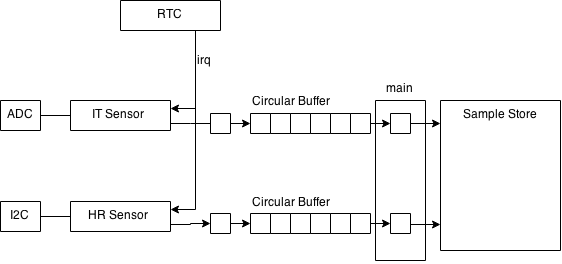
\includegraphics[scale=0.5]{figures/project-i.png}
  \end{center}
  \caption{Sample Collection Phase}
  \label{fig:project:i:samples}
\end{figure}
The main part of the application, gathering the samples, was implemented as described in \autoref{fig:project:i:samples}.
The RTC clock is set up to generate interrupts each \emph{n} milliseconds.
On each interrupt a new sample is created by the sensors and pushed into a circular buffer structure.
The main loop, which is executed once after each interrupt has been handled, extracts all the sample currently in the circular buffer and stores them in a sample store in \gls{ram}.

The sensors used in the application are shown in \autoref{tab:project:i:sensors}.

\begin{table}[H]
  \centering
  \begin{tabular}{ l | l | l | l | l }
    \textbf{\#} & \textbf{Name} & \textbf{Part} & \textbf{Connection} & \textbf{Measured Data} \\
    \hline
    0 & Internal Temperature Sensor & & ADC0 & CPU Temperature \\
    1 & Humidity Relative Sensor & Si7013 & I2C1 & Room Humidity \\
    2 & Temperature Sensor & Si7013 & I2C1 & Room Temperature \\
    \hline
  \end{tabular}
  \caption{Sensors used by the {\tracker}}
  \label{tab:project:i:sensors}
\end{table}

\paragraph{Sample Transfer}

The sample transfer mode is implemented by a \gls{cli} over the UART serial communication protocol.
The \gls{cli} offers a read command which is used to read all the samples collected from one of the three sensors described in \autoref{tab:project:i:sensors}

\subsubsection{Operation}

The {\tracker} has two interfaces for operating the application.
A manual mode switch using the buttons on the STK and a \gls{cli} interface when connected to a PC.

\paragraph{Application Modes}
The mode of operation is set by using the push buttons on the STK (a picture of the STK is found in \autoref{fig:efm32gg-stk3700}).
The operation of the buttons are shown in \autoref{tab:project:i:buttons}.

\begin{table}[H]
  \centering
  \begin{tabular}{l|l|l}
    \textbf{Currnet Mode} & \textbf{Button Pressed} & \textbf{Action} \\
    \hline
    Collect & PB0 & Go to Transfer \\
    Collect & PB1 & Stay in Collect \\
    Transfer & PB0 & Stay in Transfer \\
    Transfer & PB1 & Go to Collect after current transfer \\
    \hline
  \end{tabular}
  \caption{}
  \label{tab:project:i:buttons}
\end{table}

\paragraph{Connecting to the STK}
When the application is in transfer mode, it is controlled by a \gls{cli} connected to over UART.
To connect to the STK in transfer mode a USB cable with and FTDI chip\footnote{Future Technology Devices International provides chips for serial to USB conversion} can be used.
Connect the RX (green) and TX (white) wires as shown in \autoref{fig:project:i:connect}

\begin{figure}[H]
  \begin{center}
    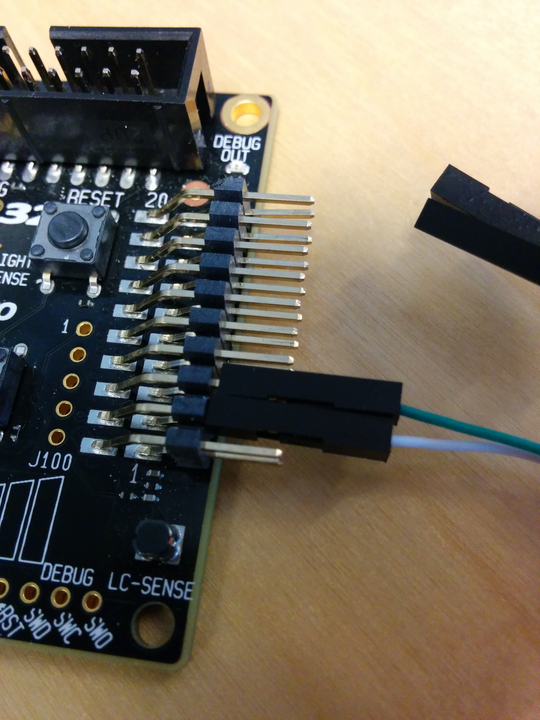
\includegraphics[scale=0.3]{figures/project-i-connect.png}
  \end{center}
  \caption{Connecting to the STK}
  \label{fig:project:i:connect}
\end{figure}

When a USB cable with FTDI is connected to the STK as shown in \autoref{fig:project:i:connect} a file handle for the serial port will be available under the \dir{/dev/} directory of a Unix like operating system.
The application can then be interacted with, with a terminal application like \prog{picocom}\footnote{\prog{picocom} is a serial terminal commonly found in many Unix-like systems}.
Connecting to the device with baudrate 9600 and error correction set to 8-1 (the defaults of \prog{picocom}) will provide access to the {\tracker} \gls{cli}.

\paragraph{Command Line Interface}
The \gls{cli} of the {\tracker} application contains a single command, read.
The read command takes one argument and is on the format \cmd{r n}, where \emph{n} is the integer 0, 1 or 2.
A read command is terminated by a carriage return, ascii symbol \code{\\n}.
All non-conforming commands are ignored by the application.
The \emph{n} parameter select the sensor data for \autoref{tab:project:i:sensors} which are queried.
Each time a command conforming command is sent the application will respond by outputting all collected samples separated by a space.

An example run of the \gls{cli} is shown in \autoref{lst:project:i:sample-run} with comments.

\begin{listing}[H]
  \begin{minted}{bash}
> r 3 // non-conformant command ignored
> r 0 // read Internal Temperature sensor
-- insert data here --
> r 0 // read Internal Temperature sensor
-- insert data here --
> r 1 // read Humidity Relative sensor
-- insert data here --
> // prompt ready for next command
  \end{minted}
  \caption{Example run of Command Line Interface}
  \label{lst:project:i:sample-run}
\end{listing}

%\subsubsection{Discussion}
